\newpage
\subsection{Implementation of the embedded server}
Here will be STM32 server implementation.


\subsubsection{Authentication and Authorization}
\paragraph{Need of security}
Users are essential part of every system. System shold be designed with
a requirement, that there will be at least one user. System without any users
does not make sense. Usually information systems have lots of users with
different roles. There should be an system administrator - the most authorized individual
in the system, managers and normal users. System should distinct them all
somehow.

Another requirement is system and information security. System may contain
sensitive data, that should not be available to general users. In case of remote
services there are some services that are not open. These services or some
of their parts are require some identity to pass through. 

Let's take a usual website as example. Common website has at least three
different user roles:
user or guest, content publisher and system administrator. Last two roles may be
joined together, but in general content publishers do not do system maintenance, they
just work with content of webpages. There may be more different roles, but these
are the main ones. Imagine you open a web page and you see the content. You
follow the links and surf the web site. If you want to change something, for
example you do not like the design or some words on web page were misspelled,
you need to find special place where you can input your \textbf{credentials} and
get into the system. This will happen only if you have proper
\textbf{permission} to do that. When you get inside you are still not able to do
anything due to lack of privileges. For example you cannot turn of the
webserver or disable the your website. There may be lots of different roles and
responsibilities in the system and each role has limited access to system
resources.

Embedded device as a service may be similar to system example above. Device may
have some limited use cases, that are not available to not authorized service
clients. This may be internal information retrieving, some  device
manipulation functions (turn on/off something, delete/remove something from the
system, change of system preferences). Some device functionality may be
available only for limited people, for example system owner. The real life example of such system is the wireless
router. Router clients are other computers, they can send and receive network
packets. Router uses wireless security protocols, which permit unauthorized
access. Even if you are connected to a secure access point, you are not able to
change system settings. You should have admin permission (password) to manage
the system. This kind of system, like many embedded systems, is made for one
purpose. Router purpose is to provide access for the network. You also can
remember lots of similar systems, that use authorized access. Nowadays it is not new to get
remotely into some device and to change internals, but embedded system
integrations are still not so common. Imagine near future, you are sitting at
work and thinking to go home. After a long day you became really hungry. You
take your smartphone and connect to your remote wireless fridge service at home. You type
your password and get list of all food in your fridge. Now you know what you
need to buy and the real candidates to be throwed to the rubbish bin. You adjust
power in some fridge area and your beer will be very cold when you get home. Is
it just a dream? Is it really hard to realize using present time technologies?


The main problem here is the security. Nowadays lots of communication between
different systems goes through the wireless channel. Radio link is also
available to your neighbour behind the wall. Generally, you do not want to
broadcast what is in your fridge or to give ability to connect to your air
conditioning service. Therefore you need to use some authentication scheme for
your service.

\paragraph{Authentication protocols}

Authentication is any process by which you verify that someone is who they claim
they are. (https://httpd.apache.org/docs/2.2/howto/auth.html)

Humanity has already invented a lot of different authentication techniques. 

The ways in which someone may be authenticated fall into three
categories: (http://en.wikipedia.org/wiki/Authentication)
\begin{itemize}
  \item the ownership factors: Something the user has (e.g., wrist band, ID
  card, security token, software token, phone, or cell phone)
  \item the knowledge factors: Something the user knows (e.g., a password, pass
  phrase, or personal identification number (PIN), challenge response (the user must answer a question), pattern)
  \item the inherence factors: Something the user is or does (e.g., fingerprint,
  retinal pattern, DNA sequence (there are assorted definitions of what is sufficient), signature, face, voice, unique bio-electric signals, or other biometric identifier).
\end{itemize}

Authentication may be one way (only client is checked for validity) and two way
( both client and server check each other). Some systems  may requre to use
different security factors together: you say password, provide ID card and show
you fingerprint There are also available many standart authentication protocols.
If you start searching you will probably find similar list:
\begin{itemize}
  \item Transport Layer Security (TLS)
  \item Extensible Authentication Protocol (EAP)
  \item Password authentication protocol (PAP)
  \item Challenge-Handshake Authentication Protocol (CHAP)
  \item Password-authenticated key agreement
  \item Remote Authentication Dial In User Service (RADIUS)
  \item Kerberos
  \item Lightweight Extensible Authentication Protocol (LEAP)  
\end{itemize}

Choosing suitable protocol is not trivial problem. There is no any case general
protocol.  Most of them are designed to interconnect big computers inside a
network. Mostly they operate on transport and application level and use TCP/IP
protocol stack.

All these protocols could be devided into these groups:
\begin{itemize}
  \item Protocols that transmit the secret over the network. (For example
  Password authentication protocol). These protocols are not secure.
  \item Protocols that not send secrets and provide authentification through
  sending messages. (CHAP and Password-authenticated key agreement).
  \item Protocols that require a trusted third party.  
\end{itemize}

Protocols of first type have been deprecated because of security reasons. They
send sensitive data over the network and everyone else between two nodes can
catch this data.

Second group of protocols was invented because the first group was unable to
provide proper level of security. Link between client and server (two parties)
does not contain pure information about the secret. Parties use cryptography and
send encrypted messages to each other. Finally they authenticate each other when there is enough information gathered to validate the authority.

Last group uses trusted third party authority to check each other. There is
assumption that all three parties should have connection between each other. Embedded device during
client authentification needs to connect some server and ask for a secret. Third
party should always have a high authority, two other parties should trust him.
This scheme should be used in case of high security requirements.



Choosing of right authentication protocol in general should depend on application. Sometimes, there even will be enough to send plain text passwords over the network. Engineer should analyze all hazards during system design process.

Lifecycle of an embedded system is more longer than livecycle of average personal computer. Application specific controller  may run for decades and it will be still functional.
Choosed security algorithm may be not secure enough after some years. Some vulnerabilities can be discovered during that period. 
Computational power of modern processors raises every year and  secure encryption may be cracked during some seconds in the future.
There is no 100% secure system, everything is breakable. 

Your system security should have such encryption, that provides proper security level to your application data and can not be cracked quickly.

Another aspect is the complexity of cryptography algorithms. Embedded devices are usually small low power devices with limited computation abilities. Not every algorithm suits well. It should be quick and in same time be secure.

Code footprint here.

Challenge-Handshake Authentication Protocol will be used in this work




 One solution is to use closed encrypted proprietary
protocol and be calm, but as it was mentioned earlier, it limits the possibility of integration
between other embedded systems. It this case all of your devices should support
that protocol and you choise of different hardware is limited. Proprietary
protocols are often vendor-specific, code is closed, documentation is not free
and all it works only with the proprietary devices from the manufacturer.


\begin{center}
 \begin{figure}[h]
	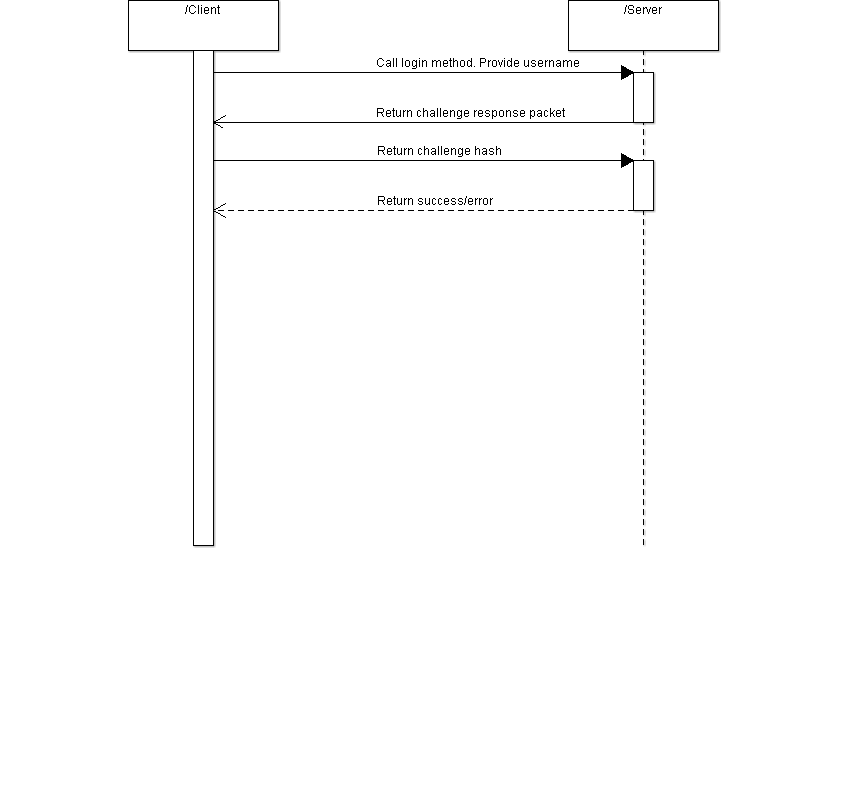
\includegraphics[width=\textwidth]{../images/implementation/embedded_server/SequenceDiagram.png}
	\caption{Client authentification process}
	\label{fig:embedded_server_login_auth}
 \end{figure}
\end{center}


